\section*{5. Results Summary}
All modules and test benches compiled without errors. ``Simulated'' values are read from the waveforms; ``Expected'' values are calculated from the equations in Section 2.

% 截圖原檔是整個 ModelSim 視窗 (1920x1040)，用 trim/clip 只裁出需要的區域，不改動原圖
% trim = 左 下 右 上 (單位 bp，PNG 無 DPI 資訊時 1 px = 1 bp)

% ------------------------------------------------------------------
\subsection*{Exp-5a: Combinational Circuit}
\begin{figure}[H]
    \centering
    \begin{minipage}[t]{0.42\textwidth}
        \vspace{0pt}
        \centering
        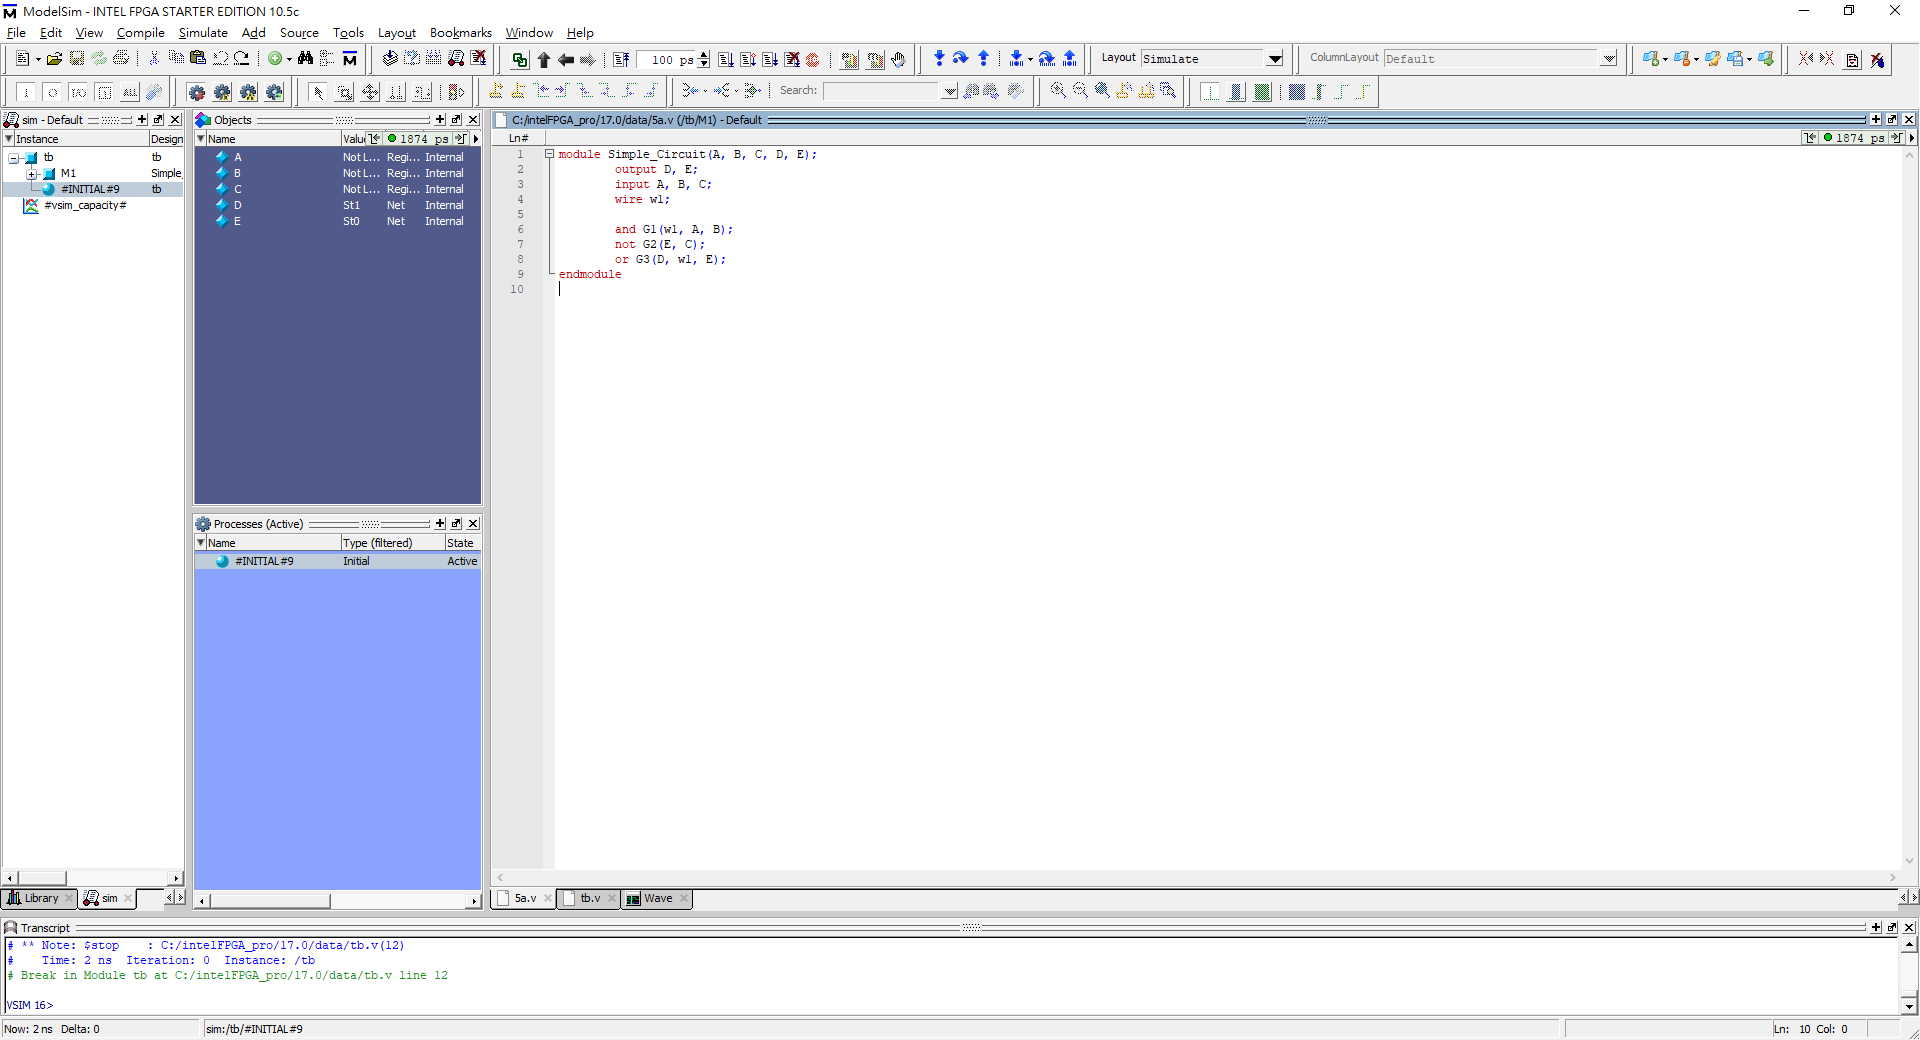
\includegraphics[width=\linewidth, trim=493 740 1020 112, clip]{pic/a1.png}
        \captionof{figure}{\texttt{5a.v} (module \texttt{Simple\_Circuit})}
        \label{fig:5a_code}
    \end{minipage}
    \hfill
    \begin{minipage}[t]{0.54\textwidth}
        \vspace{0pt}
        \centering
        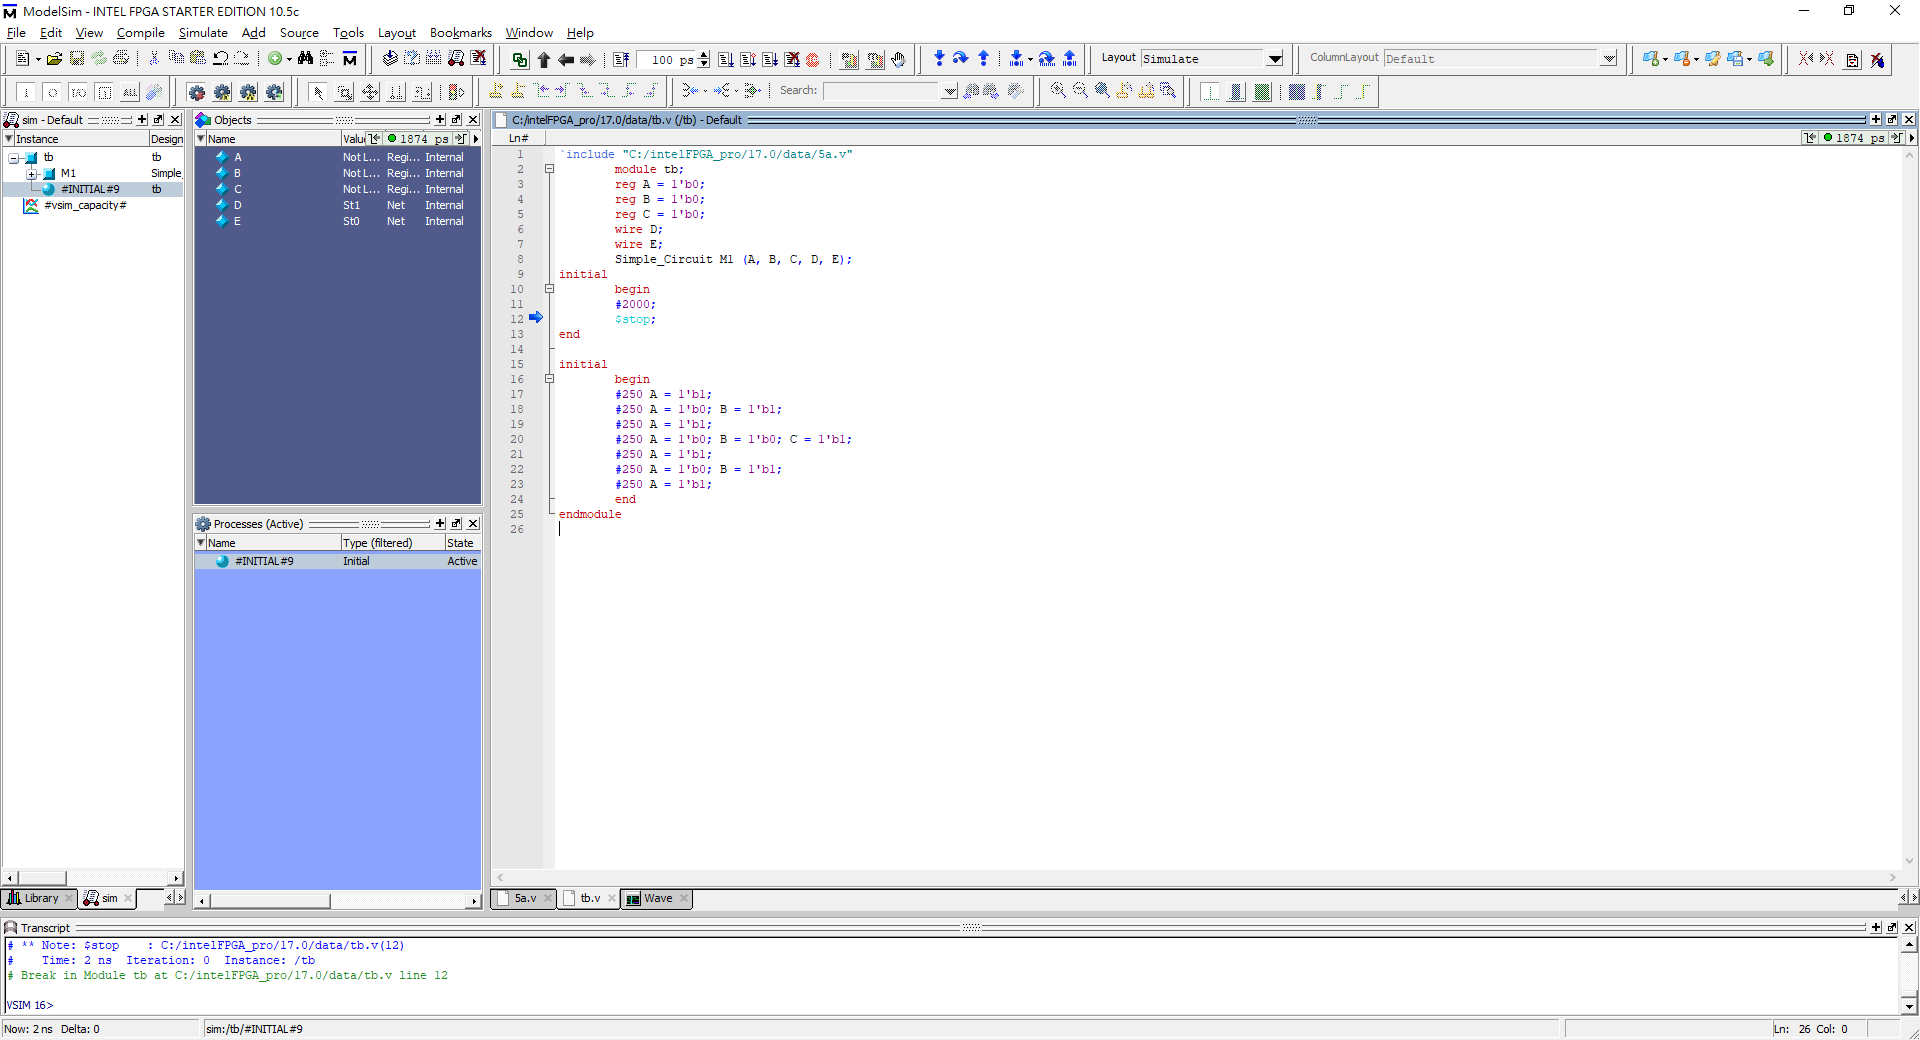
\includegraphics[width=\linewidth, trim=493 505 1020 112, clip]{pic/a2.png}
        \captionof{figure}{Test bench \texttt{tb.v} (module \texttt{tb})}
        \label{fig:5a_tb}
    \end{minipage}
\end{figure}

\begin{table}[H]
\centering
\small
\begin{tabular}{c | c c c | c c c | c c c}
\toprule
\multirow{2}{*}{\textbf{Time (ps)}} & \multicolumn{3}{c|}{\textbf{Inputs}} & \multicolumn{3}{c|}{\textbf{Expected}} & \multicolumn{3}{c}{\textbf{Simulated}} \\
 & $A$ & $B$ & $C$ & $w_1$ & $D$ & $E$ & $w_1$ & $D$ & $E$ \\
\midrule
0 -- 250     & 0 & 0 & 0 & 0 & 1 & 1 & 0 & 1 & 1 \\
1000 -- 1250 & 0 & 0 & 1 & 0 & 0 & 0 & 0 & 0 & 0 \\
500 -- 750   & 0 & 1 & 0 & 0 & 1 & 1 & 0 & 1 & 1 \\
1500 -- 1750 & 0 & 1 & 1 & 0 & 0 & 0 & 0 & 0 & 0 \\
250 -- 500   & 1 & 0 & 0 & 0 & 1 & 1 & 0 & 1 & 1 \\
1250 -- 1500 & 1 & 0 & 1 & 0 & 0 & 0 & 0 & 0 & 0 \\
750 -- 1000  & 1 & 1 & 0 & 1 & 1 & 1 & 1 & 1 & 1 \\
1750 -- 2000 & 1 & 1 & 1 & 1 & 1 & 0 & 1 & 1 & 0 \\
\bottomrule
\end{tabular}
\captionof{table}{Exp-5a truth table vs.\ simulation}
\label{tab:5a}
\end{table}

\begin{figure}[H]
    \centering
    % 上段：訊號名稱與波形；下段：時間軸（中間全黑的空白區裁掉）
    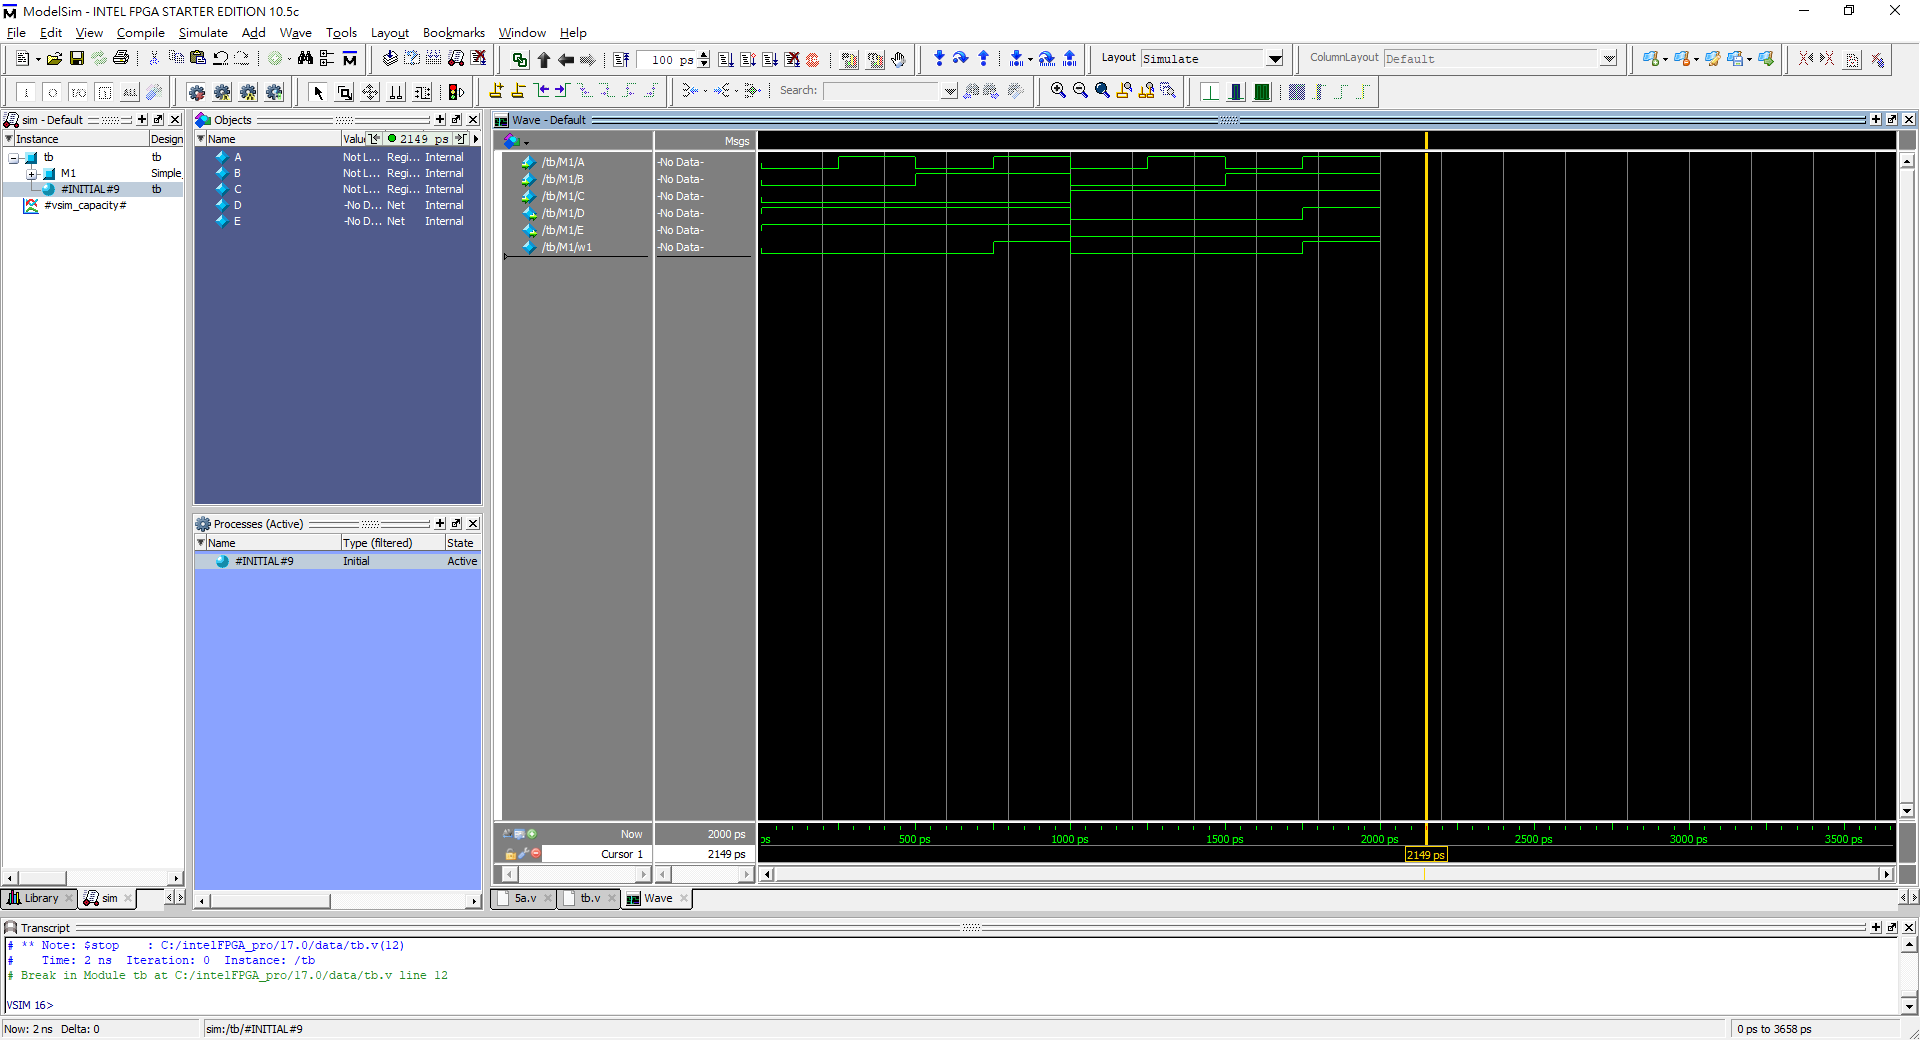
\includegraphics[width=\textwidth, trim=497 778 528 112, clip]{pic/a3.png}\\[-1pt]
    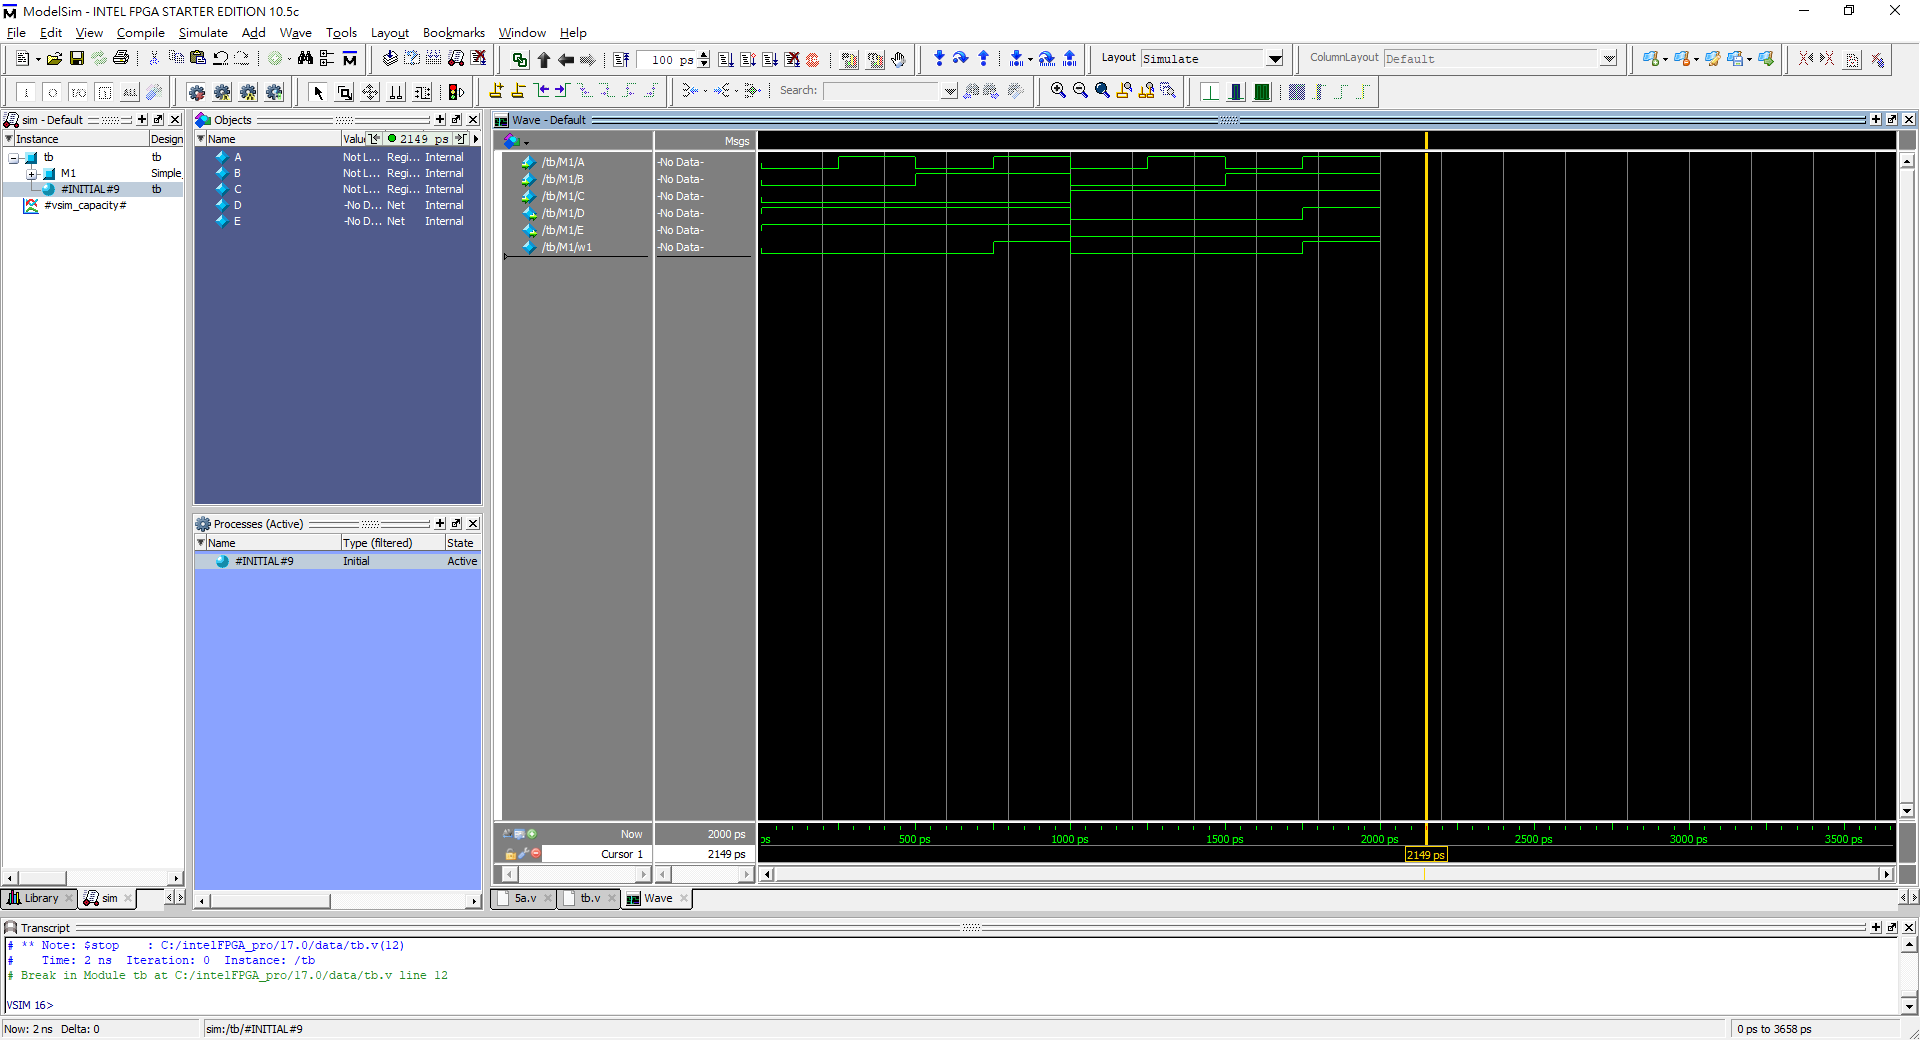
\includegraphics[width=\textwidth, trim=497 174 528 822, clip]{pic/a3.png}
    \captionof{figure}{Exp-5a simulation waveform}
    \label{fig:5a_wave}
\end{figure}

% ------------------------------------------------------------------
\subsection*{Exp-5b: Boolean Function}
\begin{figure}[H]
    \centering
    \begin{minipage}[t]{0.42\textwidth}
        \vspace{0pt}
        \centering
        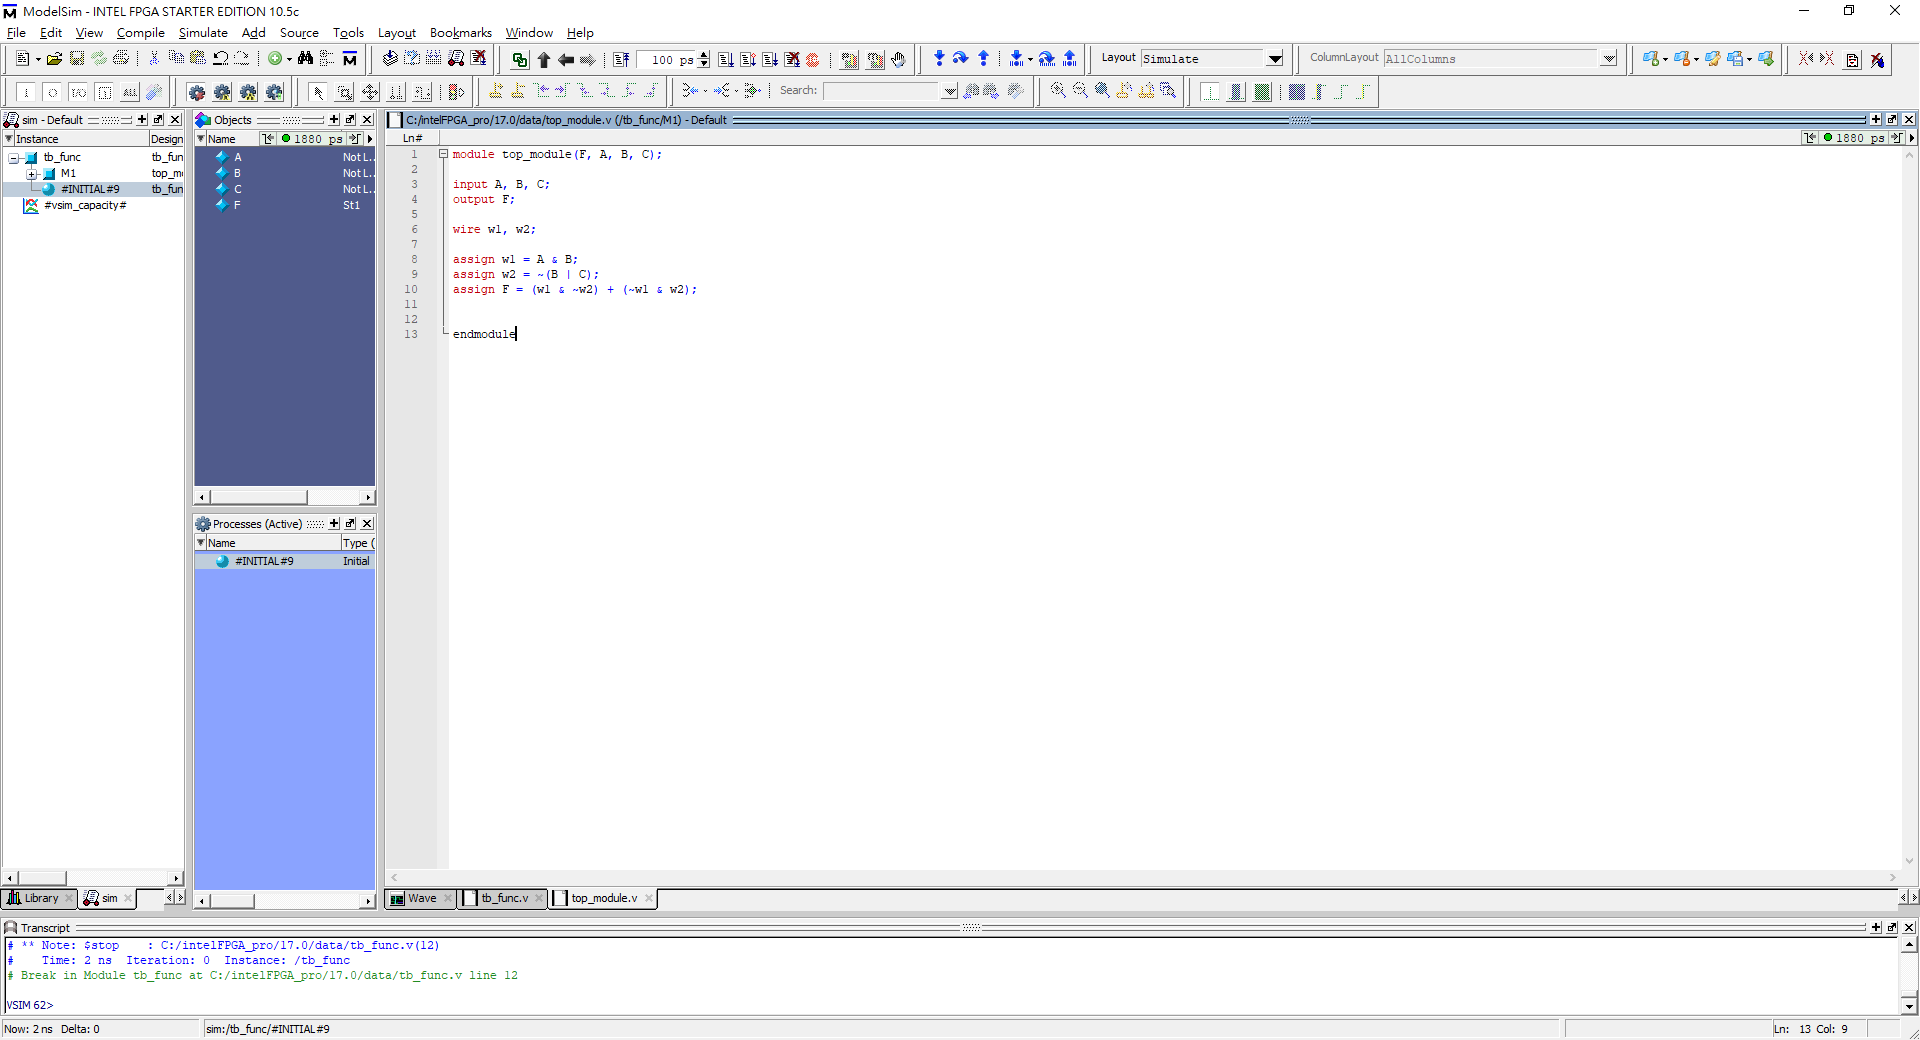
\includegraphics[width=\linewidth, trim=385 695 1160 112, clip]{pic/b1.png}
        \captionof{figure}{\texttt{top\_module.v}}
        \label{fig:5b_code}
    \end{minipage}
    \hfill
    \begin{minipage}[t]{0.54\textwidth}
        \vspace{0pt}
        \centering
        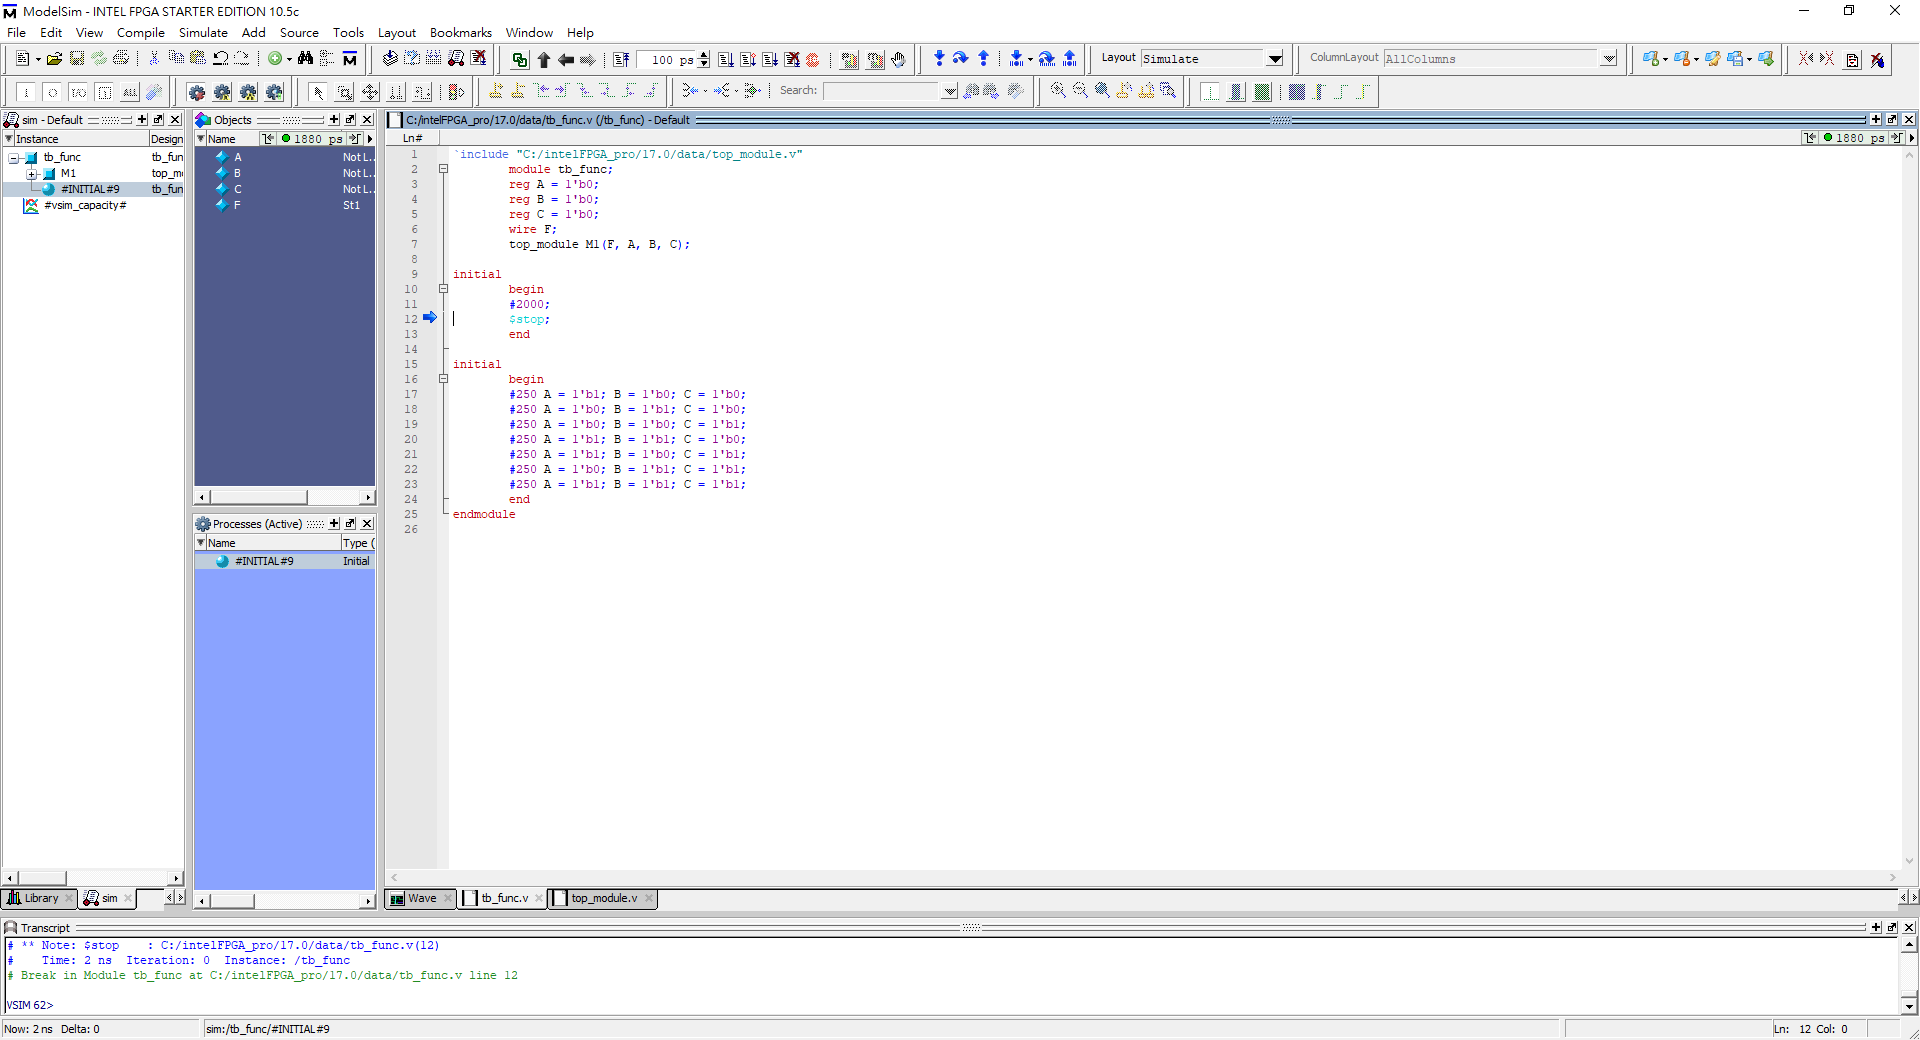
\includegraphics[width=\linewidth, trim=385 505 1110 112, clip]{pic/b2.png}
        \captionof{figure}{Test bench \texttt{tb\_func.v} (module \texttt{tb\_func})}
        \label{fig:5b_tb}
    \end{minipage}
\end{figure}

\begin{table}[H]
\centering
\small
\begin{tabular}{c | c c c | c c c | c c c}
\toprule
\multirow{2}{*}{\textbf{Time (ps)}} & \multicolumn{3}{c|}{\textbf{Inputs}} & \multicolumn{3}{c|}{\textbf{Expected}} & \multicolumn{3}{c}{\textbf{Simulated}} \\
 & $A$ & $B$ & $C$ & $w_1$ & $w_2$ & $F$ & $w_1$ & $w_2$ & $F$ \\
\midrule
0 -- 250     & 0 & 0 & 0 & 0 & 1 & 1 & 0 & 1 & 1 \\
750 -- 1000  & 0 & 0 & 1 & 0 & 0 & 0 & 0 & 0 & 0 \\
500 -- 750   & 0 & 1 & 0 & 0 & 0 & 0 & 0 & 0 & 0 \\
1500 -- 1750 & 0 & 1 & 1 & 0 & 0 & 0 & 0 & 0 & 0 \\
250 -- 500   & 1 & 0 & 0 & 0 & 1 & 1 & 0 & 1 & 1 \\
1250 -- 1500 & 1 & 0 & 1 & 0 & 0 & 0 & 0 & 0 & 0 \\
1000 -- 1250 & 1 & 1 & 0 & 1 & 0 & 1 & 1 & 0 & 1 \\
1750 -- 2000 & 1 & 1 & 1 & 1 & 0 & 1 & 1 & 0 & 1 \\
\bottomrule
\end{tabular}
\captionof{table}{Exp-5b truth table vs.\ simulation ($w_1 = A \cdot B$, $w_2 = B \downarrow C$)}
\label{tab:5b}
\end{table}

\begin{figure}[H]
    \centering
    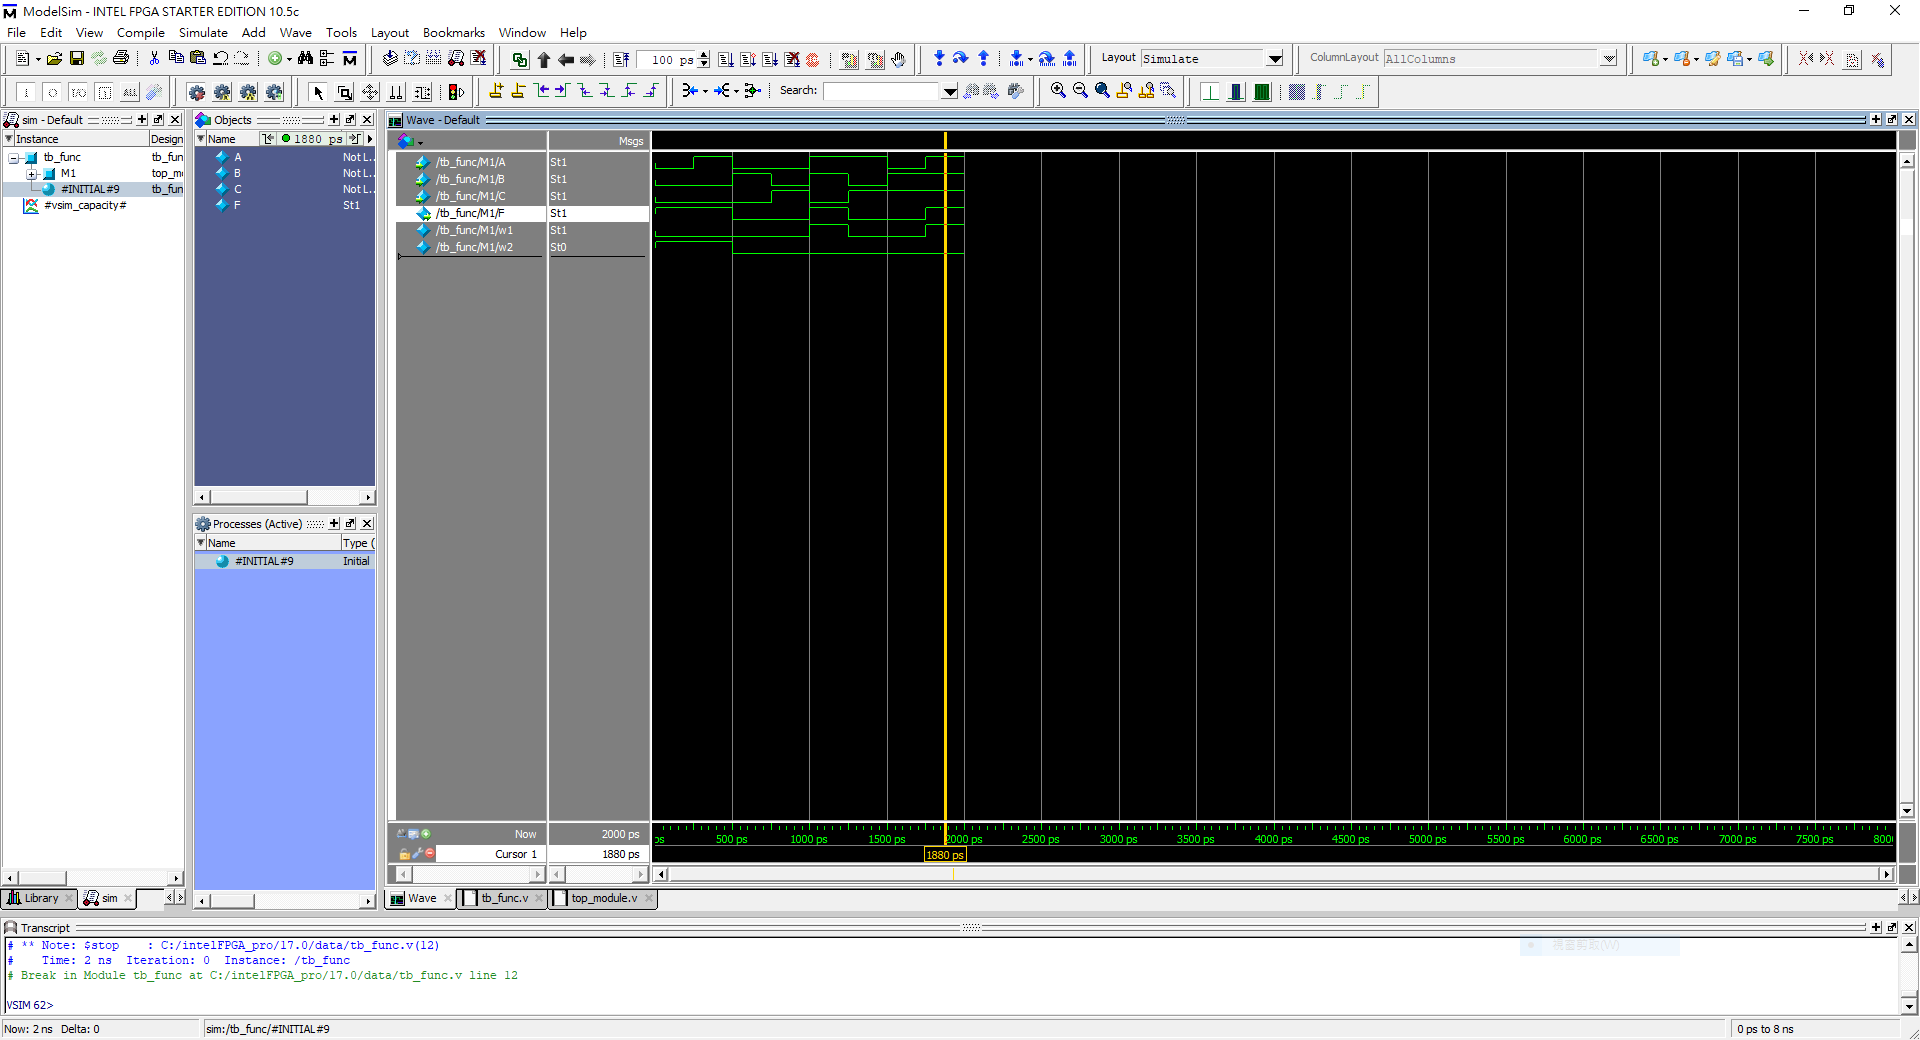
\includegraphics[width=0.75\textwidth, trim=390 778 950 112, clip]{pic/b3.png}\\[-1pt]
    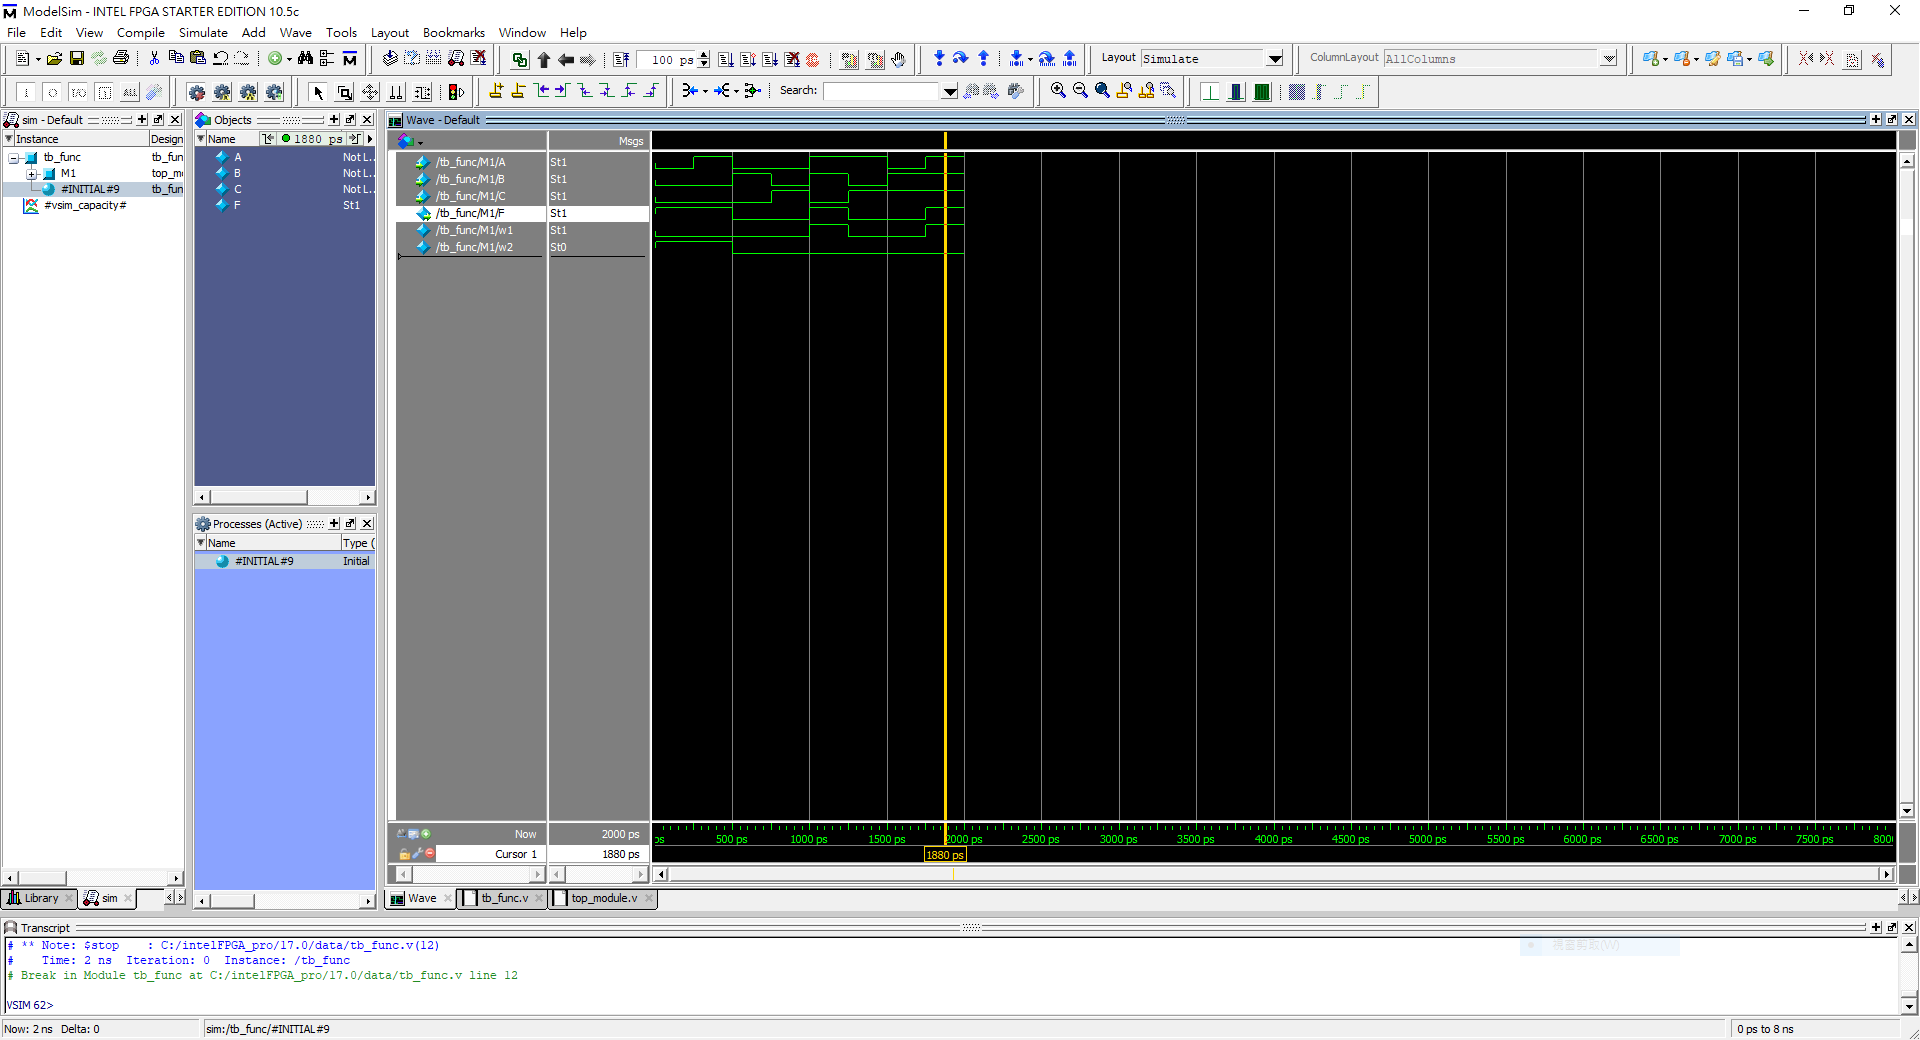
\includegraphics[width=0.75\textwidth, trim=390 174 950 822, clip]{pic/b3.png}
    \captionof{figure}{Exp-5b simulation waveform (cursor at 1880 ps: $A=B=C=1$, $w_1=1$, $w_2=0$, $F=1$)}
    \label{fig:5b_wave}
\end{figure}

For both experiments, the simulated outputs match the truth tables for all 8 input combinations.
